\documentclass{standalone}

\usepackage{pgfplots,tikz,amsmath}
\begin{document}
        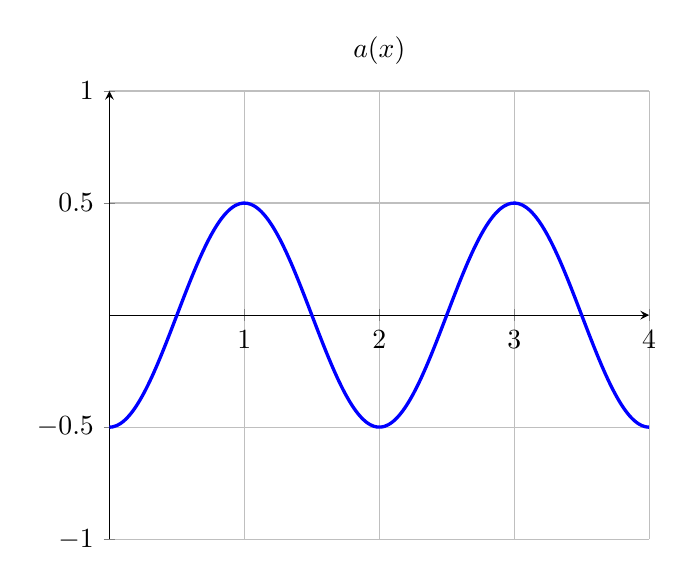
\begin{tikzpicture}
            \begin{axis}[axis lines=center, ymin=-1, ymax=1, xmin=0, xmax=4, domain=0:4,
                grid, title={$a(x)$}]
                \addplot[blue, very thick, smooth, samples=150] {0.5*cos(3.1415*(deg(x-1)))};
            \end{axis}
        \end{tikzpicture}
        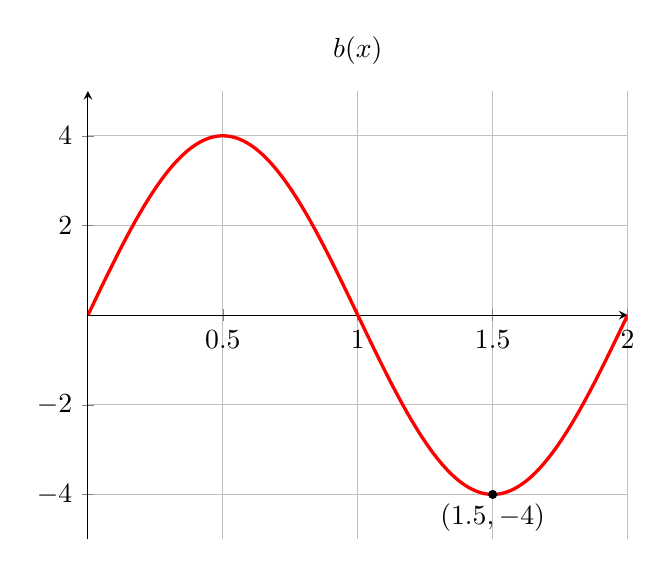
\begin{tikzpicture}
            \begin{axis}[axis lines=center, ymin=-5, ymax=5, xmin=0, xmax=2, domain=0:2,
                grid, title={$b(x)$}]
                \addplot[red, very thick, smooth, samples=150] {4*sin(3.1415*(deg(x-0)))};
                \draw[fill=black] (axis cs:1.5,-4) circle(0.05cm)
                node[anchor=north]{$(1.5,-4)$};
            \end{axis}
        \end{tikzpicture}
        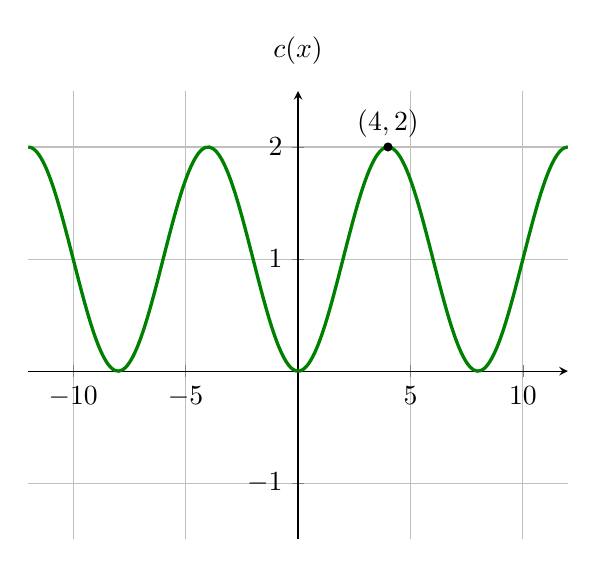
\begin{tikzpicture}
            \begin{axis}[axis lines=center, ymin=-1.5, ymax=2.5, xmin=-12, xmax=12,
                    domain=-12:12,
                grid, title={$c(x)$}]
                \addplot[green!50!black, very thick, smooth, samples=150]
                {-1*cos(3.1415/4*(deg(x-0)))+1};
                \draw[fill=black] (axis cs:4,2) circle(0.05cm) node[anchor=south]{$(4,2)$};
            \end{axis}
        \end{tikzpicture}
\end{document}
